\documentclass[tikz,border=1.5pt]{standalone}
\usepackage[T1]{fontenc}
\usepackage{lmodern}

\definecolor{ink}{HTML}{253247}
\definecolor{muted}{HTML}{657286}
\definecolor{grid}{HTML}{D7DDE7}
\definecolor{panel}{HTML}{F7F9FC}
\definecolor{blue}{HTML}{3478BF}
\definecolor{orange}{HTML}{D9822B}

\begin{document}
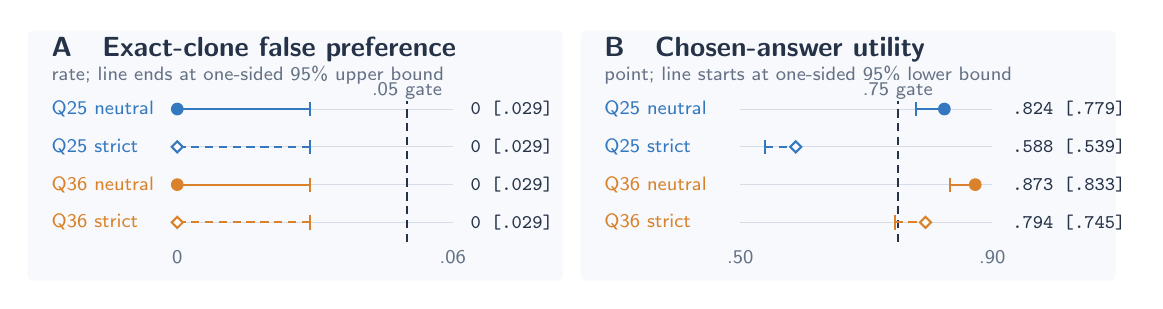
\begin{tikzpicture}[x=1cm,y=1cm,font=\sffamily\scriptsize,text=ink]
  % The same encodings are used in both panels: model by colour; criterion
  % by marker fill and line style. Direct row labels preserve grayscale use.
  \fill[panel,rounded corners=2pt] (0,0) rectangle (6.80,3.18);
  \fill[panel,rounded corners=2pt] (7.02,0) rectangle (13.82,3.18);

  \node[anchor=west,font=\sffamily\bfseries] at (0.18,2.94)
    {A\quad Exact-clone false preference};
  \node[anchor=west,text=muted] at (0.18,2.61)
    {rate; line ends at one-sided 95\% upper bound};

  \node[anchor=west,font=\sffamily\bfseries] at (7.20,2.94)
    {B\quad Chosen-answer utility};
  \node[anchor=west,text=muted] at (7.20,2.61)
    {point; line starts at one-sided 95\% lower bound};

  % Shared row labels.
  \foreach \y/\name/\col in {
    2.18/Q25 neutral/blue,
    1.70/Q25 strict/blue,
    1.22/Q36 neutral/orange,
    0.74/Q36 strict/orange} {
    \node[anchor=west,text=\col] at (0.18,\y) {\name};
    \node[anchor=west,text=\col] at (7.20,\y) {\name};
  }

  % Panel A axis: x=1.90..5.40 maps 0..0.06; fixed threshold is 0.05.
  \foreach \y in {2.18,1.70,1.22,0.74}
    \draw[grid,line width=.35pt] (1.90,\y) -- (5.40,\y);
  \draw[ink,densely dashed,line width=.55pt] (4.817,0.49) -- (4.817,2.43);
  \node[anchor=north,text=muted,fill=panel,inner sep=.7pt] at (4.817,2.55) {.05 gate};
  \node[anchor=north,text=muted] at (1.90,0.50) {0};
  \node[anchor=north,text=muted] at (5.40,0.50) {.06};

  % All four clone cells: point estimate 0, upper bound .0289428.
  \foreach \y/\col/\style in {
    2.18/blue/solid,
    1.70/blue/densely dashed,
    1.22/orange/solid,
    0.74/orange/densely dashed} {
    \draw[\col,\style,line width=.75pt] (1.90,\y) -- (3.588,\y);
    \draw[\col,line width=.75pt] (3.588,\y-.09) -- (3.588,\y+.09);
  }
  \fill[blue] (1.90,2.18) circle (2.3pt);
  \draw[blue,line width=.75pt,fill=white]
    (1.90,1.70+.07) -- (1.90+.07,1.70) -- (1.90,1.70-.07) --
    (1.90-.07,1.70) -- cycle;
  \fill[orange] (1.90,1.22) circle (2.3pt);
  \draw[orange,line width=.75pt,fill=white]
    (1.90,0.74+.07) -- (1.90+.07,0.74) -- (1.90,0.74-.07) --
    (1.90-.07,0.74) -- cycle;
  \foreach \y in {2.18,1.70,1.22,0.74}
    \node[anchor=west,font=\ttfamily\scriptsize] at (5.50,\y) {0 [.029]};

  % Panel B axis: x=9.05..12.25 maps utility 0.50..0.90.
  \foreach \y in {2.18,1.70,1.22,0.74}
    \draw[grid,line width=.35pt] (9.05,\y) -- (12.25,\y);
  \draw[ink,densely dashed,line width=.55pt] (11.05,0.49) -- (11.05,2.43);
  \node[anchor=north,text=muted,fill=panel,inner sep=.7pt] at (11.05,2.55) {.75 gate};
  \node[anchor=north,text=muted] at (9.05,0.50) {.50};
  \node[anchor=north,text=muted] at (12.25,0.50) {.90};

  % Lower bound to point estimate; neutral is solid, strict is dashed/open.
  % Qwen2.5 neutral: .779 to .824.
  \draw[blue,line width=.75pt] (11.282,2.18) -- (11.642,2.18);
  \draw[blue,line width=.75pt] (11.282,2.09) -- (11.282,2.27);
  \fill[blue] (11.642,2.18) circle (2.3pt);
  % Qwen2.5 strict: .539 to .588.
  \draw[blue,densely dashed,line width=.75pt] (9.362,1.70) -- (9.754,1.70);
  \draw[blue,line width=.75pt] (9.362,1.61) -- (9.362,1.79);
  \draw[blue,line width=.75pt,fill=white]
    (9.754,1.70+.07) -- (9.754+.07,1.70) -- (9.754,1.70-.07) --
    (9.754-.07,1.70) -- cycle;
  % Qwen3.6 neutral: .833 to .873.
  \draw[orange,line width=.75pt] (11.714,1.22) -- (12.034,1.22);
  \draw[orange,line width=.75pt] (11.714,1.13) -- (11.714,1.31);
  \fill[orange] (12.034,1.22) circle (2.3pt);
  % Qwen3.6 strict: .745 to .794.
  \draw[orange,densely dashed,line width=.75pt] (11.010,0.74) -- (11.402,0.74);
  \draw[orange,line width=.75pt] (11.010,0.65) -- (11.010,0.83);
  \draw[orange,line width=.75pt,fill=white]
    (11.402,0.74+.07) -- (11.402+.07,0.74) -- (11.402,0.74-.07) --
    (11.402-.07,0.74) -- cycle;

  \node[anchor=west,font=\ttfamily\scriptsize] at (12.38,2.18) {.824 [.779]};
  \node[anchor=west,font=\ttfamily\scriptsize] at (12.38,1.70) {.588 [.539]};
  \node[anchor=west,font=\ttfamily\scriptsize] at (12.38,1.22) {.873 [.833]};
  \node[anchor=west,font=\ttfamily\scriptsize] at (12.38,0.74) {.794 [.745]};
\end{tikzpicture}
\end{document}
